\section{Marco Teorico}

\subsection{Inteligencia Artificial}

La Inteligencia Artificial es un campo de las ciencias computacionales enfocado en el desarrollo de computadoras capaces de hacer cosas que son normalmente hechas por personas en particular, cosas asociadas con personas actuando inteligentemente.

Un investigador de la Universidad de Standford acuñó el termino en 1956 durante la que hoy se conoce como la conferencia de Dartmouth, en la cual el nucleo de la IA fue definido:

"Se intentará encontrar la manera de hacer que las máquinas utilicen el lenguaje, formen abstracciones y conceptos, resuelvan problemas que ahora están reservados a los humanos y se mejoren a sí mismas. Creemos que se puede lograr un avance significativo en uno o más de estos problemas si un grupo cuidadosamente seleccionado de científicos trabajan juntos durante un verano."

La difinicion precisa y el significado de la palabra inteligencia, y más aun de la inteligencia artificial, es el tema de mucha discusion. Un diccionario solo, por ejemplo da cuatro definiciones de Inteligencia Artificial:

\begin{itemize}
    \item Un area de estudio en el campo de la informatica. La inteligencia artificial se ocupa del desarrollo de computadoras capaces de participar en procesos de pensamiento similares a los humanos, como el aprendizaje, el razonamiento y la autocorrecion.
    
    \item El concepto de que las maquinas pueden ser imitadas asume algunas capacidades normalmente pensadas como la inteligencia humana como el aprendizaje, la adaptacion, la autocorrecion, etc.
    
    \item La extension de la inteligencia humana a traves del uso de computadoras, como en tiempos pasados, el poder fisico se extendi a traves del uso de las herramintas mecanicas.
    
    \item En un sentido restringido, el estudio de las tecnicas para utilizar las computadoras de formas mas eficaz mediante tecnicas de programacion mejoradas
    
\end{itemize}

(The New International Webster’s Comprehensive Dictionary of the English Language, EncyclopedicEdition) 

Hoy en dia la comunidad de Inteligencia Artificial ha tratado de imitar comportamientos inteligentes con programas computacionales. Esto no es una tarea facil porque un programa de computadora debe se capaz de hacer muchas maneras en orden para ser llamado inteligente.

Hay muchas mas definiciones para la Inteligencia Artificial, pero la mayoria se pueden clasificar en cuatro categorias:

\begin{itemize}
    \item Sistemas que piensan como humanos
    
    \item Sistemas que actuan como humanos
    
    \item Sistemas que piensan racionalmente
    
    \item Sistemas que actuan racionalmente
\end{itemize}


\subsection{Aprendizaje Automatico}
El Aprendizaje Automatico es la ciencia de la programacion de las computadoras en la cual purden aprender de deteccion automatizada de patrones significativos en datos.

\textbf{Una ligera definicion:}

El aprendizaje automatico es el campo de estudio que le da a las computadoras la habilidad de aprender sin ser explicitamente programadas

-Arthur Samuel, 1959

\textbf{Una definicion mas en terminos de Ingenieria:}

Un programa computacional es dicho para aprender de la experiencia E con respecto a alguna tarea T y algo de medida de rendimiento P, si su rendmiento en T, por medio de P, mejorada con la experiencia E.

-Tom Mitchell, 1997

\textbf{Aplicaciones del Aprendizaje Automatico: }

\begin{itemize}
    \item Ranqueo de paginas: Esto es, el proceso de enviar una consulta a un motod de busquea, que luego encuentra las paginas web relevantes para la consulta y que las devuelve en su orden de relevancia. El aprendizaje automatico en lugar de se utiliza para automatizar el proceso de diseño de un buen motor de busqueda.
    
    \item Filtracion Colaborativa: Las compañias electronicas que ofrecen musica y pelicuas en streamming como Amazon o Netflix usan la informacion extensamente para convencer a los usuarios de comprar contenido en base a su informacion.
    
    \item Traduccion automatica de documentos: En un extremo, nosotros podemos enfocar un completo entendimiento de un texto antes de traducirlo usando un conjunto de reglas seleccionadas por un linguista computacional bien versado en los dos idiomas que nos gustaria traducir
    
    \item Muchas aplicaciones de seguridad: por ejempo el control de acceso, usando patrones de reconocimiento como uno de sus componentes. ESto es dando una foto (o grabando un video) de una persona, reconociendo quien es esta persona. En otras palabras, el sistema necesita clasificar las caras dentro de una de muchas categorias (Alicia, Bob, Carlos) o decidir que es una cara desconocida.
    
\end{itemize}

\textbf{Aprendizaje Automatico es bueno en:}

\begin{itemize}
    \item Problemas para los que las soluciones existentes requieren de mucho ajuste manual o largas listas de reglas: un algoritmo de Aprendizaje Automatico a menudo puede simplificar el codigo y rendir mejor
    
    \item Problemas complejos para los cuales no existe una buena solucion utilizando un enfoque tradicional: las mejores tecnicas de Aprendizaje Automatico pueden encontrar una solucion
    
    \item Entornos fluctantes: un sistema de Aprendizaje Automatico puede adaptarse a nuevos datos
    
    \item Obtener informacion sobre problemas complejos y grandes cantidades de datos
    
\end{itemize}

\textbf{Tipos de sistemas de Aprendizaje Automatico:}

Hay varios tipos de diferentes sistemas basados en apendizaje automatico que se pueden clasificar en las siguiente categorias:

\begin{itemize}

    \item Si estan o no entrenados con supervision humana (supervisados, no supervisados, semisupervisados y aprendizaje por refuerzo)
    
    \item Si pueden o no apredner gradualmente sobre la marcha (aprendizaje en linea versus aprendizaje por lotes)
    
    \item  Ya sea que trabajen simplemente comparando nuevos puntos de datos con puntos de datos conocidos, o en su lugar detecten patrones en los datos de entrenamineto y contruyan un modelo predictivo, de manera muy parecida a como lo hacen los cientificos (aprendizaje basado en instancias versus aprendizaje basado en modelos)
    
\end{itemize}

Los sistemas de aprendizaje automatico pueden ser clasificados de acuerdo a la cantidad y tipos de supervision que reciben durante el entrenamiento. Hay cuatro principales categorias: aprendizaje supervisado, aprendizaje no supervisado, aprenizaje semisupervisado y aprendizaje por refuerzo.

\subsection{Aprenizaje Supeervisado}
En el aprenizaje supervisado, los datos de entrenamiento que alimentan al algoritmo incluyen las soluciones deseadas llamadas etiquetas.

\begin{figure}[ht]
	\centering
	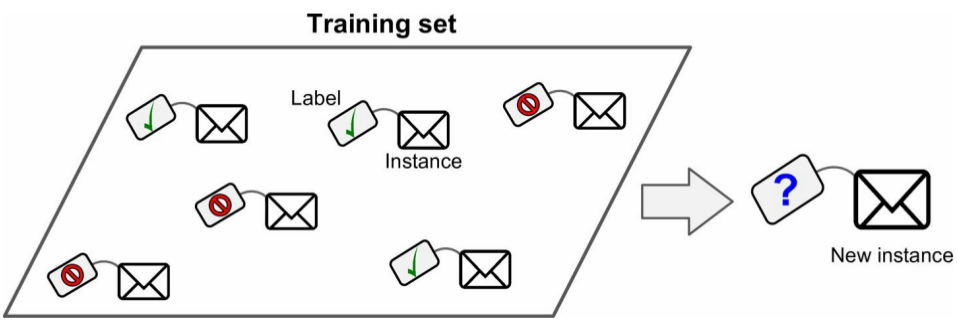
\includegraphics[width=0.30\linewidth]{figuras/supervisedLearning.png}
	\caption{Aprendizaje supervisado}
	\label{AS}
\end{figure}

Una tipica tarea en el aprendizaje supervisado es la clasificacion. El filtrador de spam del correo electronico es un buen ejemeplo de esto: este se entrena con muchos ejemplos de correos electronicos junto con su clase (spam o no spam), y debe aprender a clasificar los nuevos correos electronicos.

\textbf{Algoritmos de Aprendizaje Supervisado}  \\
\begin{itemize}
    \item K-Nearest Neighbors
    
    \item Regresion Lineal
    
    \item Refresion Logica
    
    \item Máquinas de Vectores de Soporte
    
    \item Arboles de decision y bosques aleatorios
    
    \item Redes Neuronales
    
\end{itemize}

\subsection{Aprendizaje no supervisado}
En el aprendizaje no supervisado, los datos de entrenamiento no estan etiquetados. Los sistemas intentan aprender sin un maestro.

\begin{figure}[ht]
	\centering
	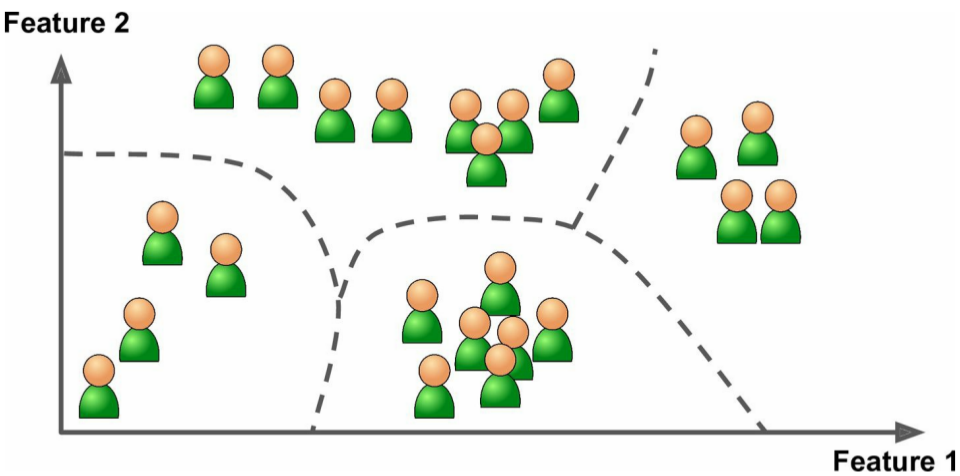
\includegraphics[width=0.30\linewidth]{figuras/clustering.png}
	\caption{Aprendizaje No Supervisado}
	\label{ANS}
\end{figure}

\textbf{Algoritmos de Aprendizaje No Supervisado} 

\begin{itemize}
    \item Agrupamiento
    	\begin{itemize}
    		\item K-Means
   			\item Hirerchical Cluster Analysis (HCA)
    		\item Expectation Maximization
		\end{itemize}
    \item Visualizacion y reduccion de la dimensionalidad
    	\begin{itemize}
    		\item Principal Component Analysis (PCA)
   			\item Kernel PCA
    		\item Locally-Linear Embedding (LLE)
    		\item t-distributed Stochastic Neighbor Embedding (t-SNE)
		\end{itemize}
    \item Aprendizaje de las reglas de asociacion
    	\begin{itemize}
    		\item Apriori
   			\item Eclat
		\end{itemize}
\end{itemize}

\subsection{Aprendizaje Semisupervisado}

Algunos algoritmos pueden tratar con datos de entrenamiento parcialmente etiquetados, normalmente muchos datos sin etiquetar y un poco de datos etiquetados. Esto se llama aprendizaje semisupervisado. Algunos servicios de alojamiento de fotos, como Google Photos, son buenos ejemplos de ello. Una vez que cargues todas tus fotos familiares en el servicio, reconocerá automáticamente que la misma persona A aparece en las fotos 1, 5 y 11, mientras que otra persona B aparece en las fotos 2, 5 y 7. Esta es la parte no supervisada del algoritmo (clustering). Ahora todo lo que el sistema necesita es que le digas quiénes son estas personas. Sólo una etiqueta por persona, 4 y es capaz de nombrar a todos en cada foto, lo que es útil para buscar fotos.

\begin{figure}[ht]
	\centering
	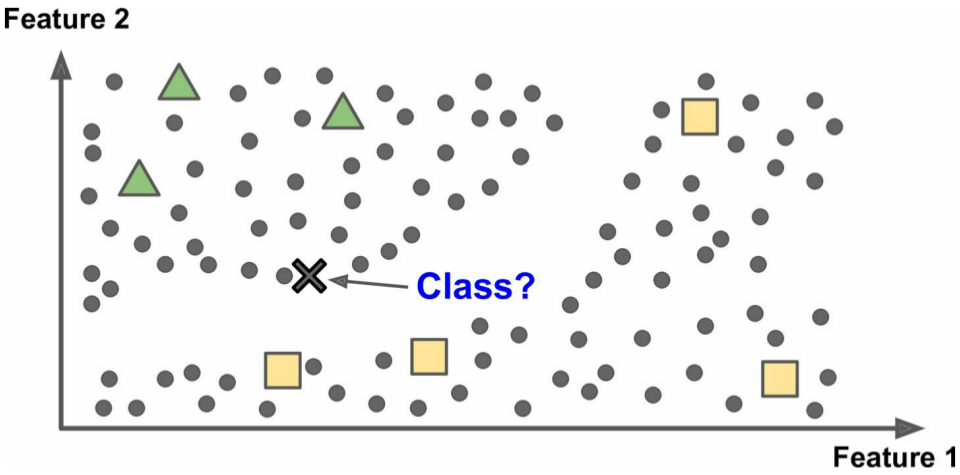
\includegraphics[width=0.30\linewidth]{figuras/semisupervised.png}
	\caption{Aprendizaje Semisupervisado}
	\label{ASS}
\end{figure}

La mayoría de los algoritmos de aprendizaje semisupervisados son combinaciones de algoritmos supervisados y no supervisados. Por ejemplo, las redes de creencias profundas (DBN, por sus siglas en inglés) se basan en componentes no supervisados llamados máquinas Boltzmann restringidas (RBM, por sus siglas en inglés) apiladas unas encima de otras. Los mecanismos para encuadernación con anillos se capacitan secuencialmente de manera no supervisada, y luego se perfecciona todo el sistema utilizando técnicas de aprendizaje supervisado.


\subsection{Aprenizaje Por Refuerzo}
El Aprendizaje de Refuerzo (RL) se refiere a un tipo de método de Aprendizaje Automático en el cual el agente recibe una recompensa retardada en el siguiente paso del tiempo para evaluar su acción previa. Se utilizaba sobre todo en juegos (por ejemplo, Atari, Mario), con un rendimiento igual o incluso superior al de los humanos. Recientemente, a medida que el algoritmo evoluciona con la combinación de redes neuronales, es capaz de resolver tareas más complejas, como el problema del péndulo.

Típicamente, una configuración de RL está compuesta de dos componentes, un agente y un entorno:

\begin{figure}[ht]
	\centering
	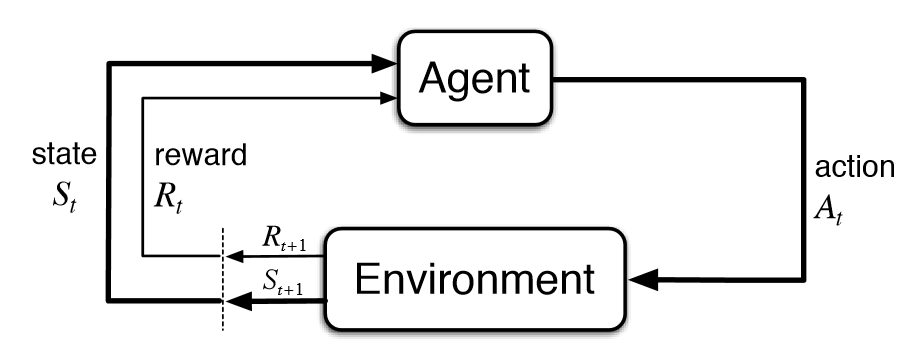
\includegraphics[width=0.30\linewidth]{figuras/reinforcementLearning.png}
	\caption{Configuracion del Aprendizaje por refuerzo}
	\label{ASS}
\end{figure}


Entonces el entorno se refiere al objeto sobre el que el agente está actuando (por ejemplo, el propio juego en el juego de Atari), mientras que el agente representa el algoritmo. El entorno comienza enviando un estado al agente, que luego se basa en su conocimiento para tomar una acción en respuesta a ese estado. Después de eso, el entorno envía un par de estado siguiente y la recompensa de vuelta al agente. El agente actualizará sus conocimientos con el premio devuelto por el medio ambiente para evaluar su última acción. El bucle continúa hasta que el entorno envía un estado terminal, que termina en episodio.

La mayoría de los algoritmos de RL siguen este patrón.

\textbf{Elementos dentro de un algoritmo de aprendizje por refuerzo: }

 \begin{itemize}
  
  \item{ } \textbf{Accion (A): } Todos los movimientos posibles que el agente puede hacer

  \item{ } \textbf{Estado (S): } Situación actual devuelta por el medio ambiente.
	 
  \item{ } \textbf{Recompenza (R): } Un retorno inmediato desde el entorno para evaluar la última acción. 
  		
  \item{ } \textbf{Politica ($\pi$): }  La estrategia que el agente emplea para determinar la siguiente acción basada en el estado actual.
  
  \item{ } \textbf{Valor (V): }  El rendimiento esperado a largo plazo con descuento, a diferencia de la recompensa a corto plazo R. V$\pi$(s) se define como el rendimiento esperado a largo plazo de la actual política de extinción del estado $\pi$.
  
  \item{ } \textbf{valor Q or accion-valor (Q): }   El valor Q es similar al valor V, excepto que toma un parámetro extra, la acción actual a. Q$\pi$(s, a) se refiere al retorno a largo plazo del estado actual s, tomando la acción a bajo la política $\pi$.
  
  \end{itemize}
  
\textbf{Libre de Modelo vs Basado en Modelo: }

El modelo representa la simulación de la dinámica del entorno. Es decir, el modelo aprende la probabilidad de transición T(s1|(s0, a)) del par de estado actual s0 y la acción a al siguiente estado s1. Si la probabilidad de transición se aprende con éxito, el agente sabrá la probabilidad de entrar en un estado específico dado el estado actual y la acción. Sin embargo, los algoritmos basados en modelos se vuelven poco prácticos a medida que crece el espacio de estado y el espacio de acción (S * S * A, para una configuración tabular).

Por otro lado, los algoritmos sin modelos se basan en pruebas y errores para actualizar sus conocimientos. Como resultado, no requiere espacio para almacenar toda la combinación de estados y acciones. Todos los algoritmos discutidos en la siguiente sección caen dentro de esta categoría.

\textbf{Con-Politica vs Sin-Politica }

Un agente con-politica aprende el valor basado en su acción actual a derivada de la política actual, mientras que su contraparte sin-politica lo aprende basado en la acción a* obtenida de otra política. En Q-learning, tal política es la política codiciosa.

\subsection{Algoritmo Q-Learning}

Q-Learning es un algoritmo de Aprendizaje Por Refuerzo libre de politicas y modelos basado en la conocida ecuacion de Bellman:

\begin{figure}[ht]
	\centering
	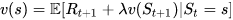
\includegraphics[width=0.30\linewidth]{figuras/bellman.png}
	\label{bellman}
\end{figure}

E en la ecuación anterior se refiere a la expectativa, mientras que $\lambda$ se refiere al factor de descuento. Podemos reescribirlo en forma de valor Q:

\begin{figure}[ht]
	\centering
	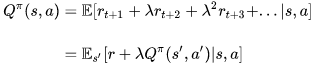
\includegraphics[width=0.30\linewidth]{figuras/qBellman.png}
	\label{qbellman}
\end{figure}

El valor óptimo de Q, indicado como Q*, puede expresarse como:

\begin{figure}[ht]
	\centering
	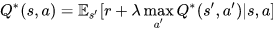
\includegraphics[width=0.30\linewidth]{figuras/qvalue.png}
	\label{qvalue}
\end{figure}

El objetivo es maximizar el valor Q.

\subsection{Redes Neuronales}

Una red neuronal artificial (RNA) es un modelo computacional basado en la estructura y funciones de las redes neuronales biológicas. La información que fluye a través de la red afecta a la estructura de la RNA porque una red neuronal cambia -o aprende, en cierto sentido- basándose en esa entrada y salida.

Las RNA se consideran herramientas de modelado de datos estadísticos no lineales en las que se modelan las complejas relaciones entre entradas y salidas o se encuentran patrones.

La RNA también se conoce como red neuronal.



Una RNA tiene varias ventajas, pero una de las más reconocidas es el hecho de que puede aprender de la observación de conjuntos de datos. De esta forma, la RNA se utiliza como una herramienta de aproximación de función aleatoria. Estos tipos de herramientas ayudan a estimar los métodos más rentables e ideales para llegar a las soluciones mientras se definen las funciones o distribuciones de computación. ANN toma muestras de datos en lugar de conjuntos de datos completos para llegar a soluciones, lo que ahorra tiempo y dinero. Las RNA se consideran modelos matemáticos bastante simples para mejorar las tecnologías de análisis de datos existentes.

Las RNA tienen tres capas interconectadas. La primera capa consiste en neuronas de entrada. Esas neuronas envían datos a la segunda capa, que a su vez envía las neuronas de salida a la tercera capa.

Entrenar una red neural artificial implica elegir entre modelos permitidos para los que existen varios algoritmos asociados.

\begin{figure}[ht]
	\centering
	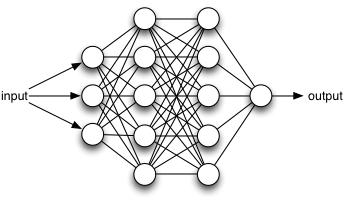
\includegraphics[width=0.30\linewidth]{figuras/neuralNetwork.png}
	\label{qvalue}
\end{figure}

\textbf{Perceptron}

Existen varios modelos para representar una red neuronal. Estos modelos difieren también en los modelos matemáticos. El modelo inicial y más sencillo de entender es el conocido como Pecepron.

Los perceptrones fueron desarrollados en las décadas de 1950 y 1960 por el científico Frank Rosenblatt.  Un perceptrón toma varias entradas binarias, $x1,x2,...,$ y produce una sola salida binaria: 

\begin{figure}[ht]
	\centering
	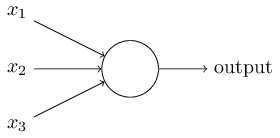
\includegraphics[width=0.30\linewidth]{figuras/perceptron.png}
	\label{qvalue}
\end{figure}

En el ejemplo mostrado el perceptrón tiene tres entradas, $x1,x2,x3.$ En general podría tener más o menos entradas. Rosenblatt propuso una regla simple para calcular el resultado. Introdujo pesos, $w1,w2,...,$ números reales que expresan la importancia de las respectivas entradas a la salida

  La salida de la neurona, 0 o 1, se determina por si la suma ponderada $\sum_{j} w_{j} x_{j} $ es menor o mayor que algún valor umbral. Al igual que los pesos, el umbral es un número real que es un parámetro de la neurona. Para ponerlo en términos algebraicos más precisos: 
  
  \begin{figure}[ht]
	\centering
	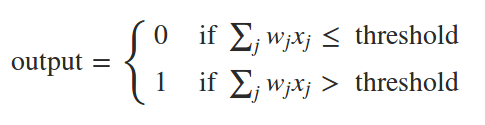
\includegraphics[width=0.30\linewidth]{figuras/perceptron_formula.png}
	\label{qvalue}
\end{figure}
  
 Simplifiquemos la forma en que describimos los preceptrones. La condición $\sum_{j} w_{j} x_{j} > threshold$  es engorroso, y podemos hacer dos cambios notacionales para simplificarlo. El primer cambio es escribir $\sum_{j} w_{j} x_{j} $ como un producto punto, $ w * x \equiv \sum_{j} w_{j} x_{j} $ donde w y x son vectores los cuales componen los pesos y las entradas, respectivamente. El segundo cambio es mover el umbral al otro lado de la desigualdad, y reemplazarlo por lo que se conoce como el sesgo del perceptrón, $ b \equiv -threshold $. Usando el sesgo en lugar del umbral, la regla del perceptrón puede ser reescrita: 
 
   \begin{figure}[ht]
	\centering
	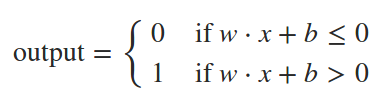
\includegraphics[width=0.30\linewidth]{figuras/perceptron_formula_2.png}
	\label{qvalue}
\end{figure}
 
Se puede pensar en el sesgo como una medida de lo fácil que es conseguir que el perceptrón emita un 1. O para decirlo en términos más biológicos, el sesgo es una medida de lo fácil que es conseguir que el perceptrón se dispare. Para un perceptrón con un sesgo realmente grande, es extremadamente fácil para el perceptrón emitir un 1. Pero si el sesgo es muy negativo, entonces es difícil para el perceptrón emitir un 1
 
 En la red de abajo, la primera columna de percepciones - lo que llamaremos la primera capa de percepciones - es tomar tres decisiones muy simples, sopesando la evidencia de entrada. ¿Qué hay de las percepciones en la segunda capa? Cada una de esas percepciones está tomando una decisión sopesando los resultados de la primera capa de la toma de decisiones. De esta manera un perceptrón en la segunda capa puede tomar una decisión a un nivel más complejo y abstracto que los perceptrones en la primera capa. Y el perceptrón de la tercera capa puede tomar decisiones aún más complejas. De esta manera, una red de múltiples capas de percepciones puede participar en la toma de decisiones sofisticadas.
 
\begin{figure}[ht]
	\centering
	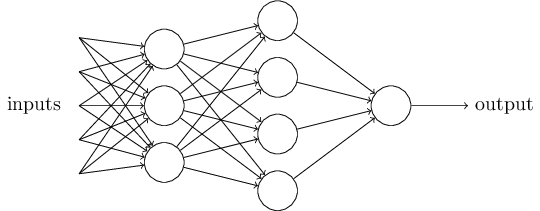
\includegraphics[width=0.30\linewidth]{figuras/net.png}
	\label{qvalue}
\end{figure}


\subsection{TensorFlow}

TensorFlow es una librería de software de código abierto para computación numérica usando gráficas de flujo de datos. Fue desarrollado originalmente por el equipo de Google Brain dentro de la organización de investigación Machine Intelligence de Google para el aprendizaje automático y la investigación de redes neuronales profundas, pero el sistema es lo suficientemente general como para ser aplicable en una amplia variedad de otros dominios también.

TensorFlow es multiplataforma. Funciona en casi todo: GPUs y CPUs -incluyendo plataformas móviles y embebidas- e incluso unidades de procesamiento tensorial (TPUs), que son hardware especializado para realizar cálculos tensores.

\textbf{Modelos de Ejecucion de TensorFlow: Ejecucion de Grafos computacionales }

El aprendizaje automático puede volverse complejo rápidamente, y los modelos de aprendizaje profundo pueden hacerse grandes. Para muchos gráficos de modelos, necesita capacitación distribuida para poder iterar dentro de un marco de tiempo razonable. 
Con Tensorflow puede escribir código para construir un gráfico de cálculo, luego ejecutarlo. El gráfico es una estructura de datos que describe completamente el cálculo que se desea realizar.

Tiene las siguientes ventajas:

  \begin{itemize}
  
  \item{ }Es portátil, ya que el gráfico puede ejecutarse inmediatamente o guardarse para su uso posterior

  \item{ }Puede funcionar en múltiples plataformas: CPUs, GPUs, TPUs, móviles, embebidos. 
  		
  \item{ }Es transformable y optimizable, ya que el gráfico puede ser transformado para producir una versión más óptima para una plataforma determinada. Además, se pueden realizar optimizaciones de memoria o de cálculo y realizar compensaciones entre ellas.  
  		 
   \item{ }Soporte para ejecución distribuida

  \end{itemize}
  
\textbf{TensorBoard}

Tensorboard es un conjunto de aplicaciones web para inspeccionar, visualizar y comprender las ejecuciones y gráficos de TensorFlow. Puede usar TensorBoard para ver las gráficas de su modelo TensorFlow y acercarse a los detalles de las subsecciones de las gráficas.
Puede trazar métricas como la pérdida y la precisión durante una ejecución de entrenamiento; mostrar visualizaciones de histogramas de cómo un tensor está cambiando con el tiempo; mostrar datos adicionales, como imágenes; recopilar metadatos de tiempo de ejecución para una ejecución, como el uso total de memoria y las formas de tensores para los nodos; y más.

\begin{figure}[ht]
	\centering
	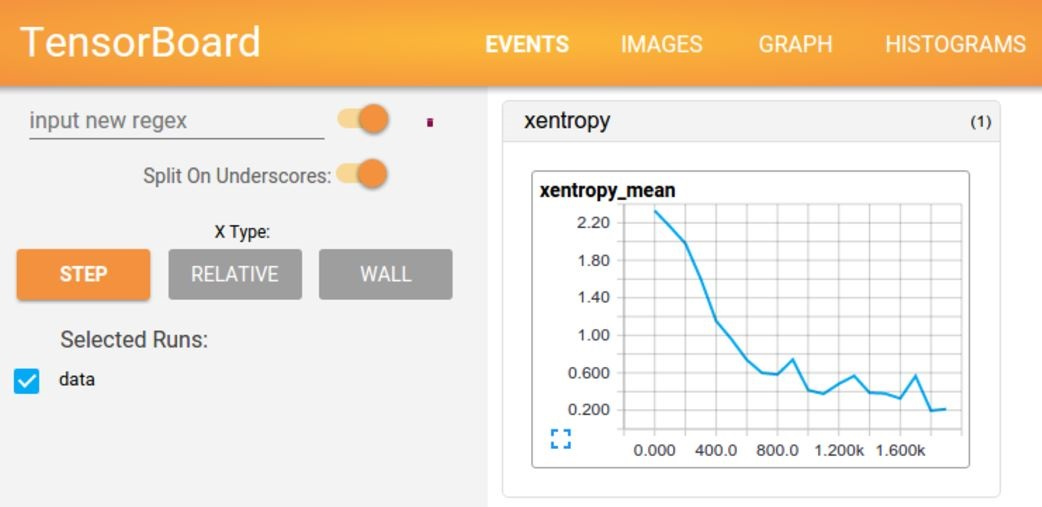
\includegraphics[width=0.30\linewidth]{figuras/tensorboard.jpg}
	\label{qvalue}
\end{figure}


\textbf{Computacion basado en Grafos:}

Tensorflow es un sistema de programación en el que los cálculos computacionales se representan en forma de gráfos. Los nodos en el grafo se llaman ops (abreviatura de operaciones) - Una operación toma cero o más tensores, realiza una cierta operación computacional y produce cero o más tensores. Un tensor es un conjunto multidimensional y estandarizado.


\begin{figure}[ht]
	\centering
	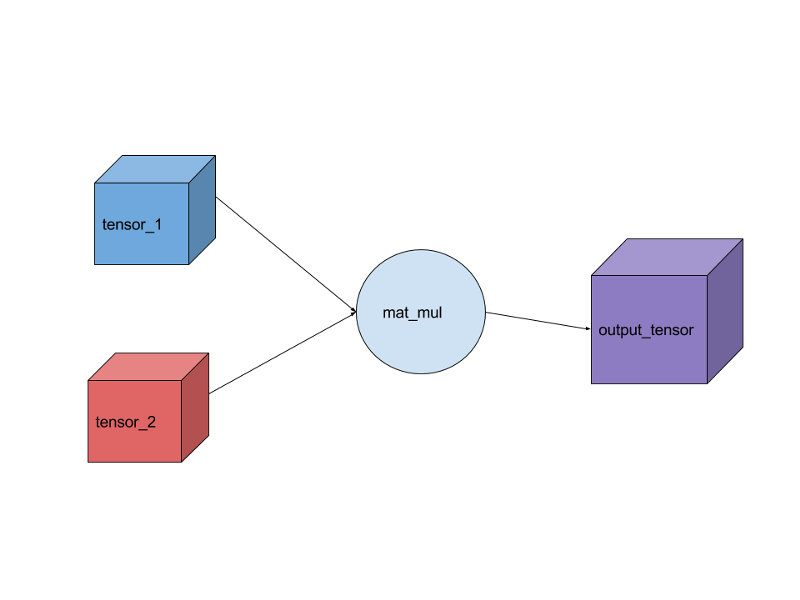
\includegraphics[width=0.30\linewidth]{figuras/tf1.png}
	\label{qvalue}
\end{figure}

Los programas Tensorflow suelen estructurarse en una fase de construcción y una fase de ejecución que utiliza una sesión para ejecutar operaciones en el gráfico.

Por ejemplo, es común crear un gráfico para representar y entrenar una red neuronal en la fase de construcción, y luego ejecutar repetidamente un conjunto de operaciones entrenadas en la fase de ejecución.

Para construir un gráfo, se parte de los ops que no requieren ninguna entrada (source ops), como una constante, y pasa su salida a otro ops para realizar el cálculo computacional.

El constructor de operaciones en la librería Python devuelve los objetos que se mantienen para la salida de las operaciones construidas. Puede pasarlos a otras operaciones construidas para usarlos como entradas.

La librería Python para TensorFlow tiene una gráfica por defecto que añade nodos a los builders ops. El gráfico por defecto es suficiente para muchas aplicaciones.

\subsection{OpenAI gym}

Gym es un juego de herramientas para desarrollar y comparar algoritmos de aprendizaje de refuerzo. No hace suposiciones sobre la estructura de su agente, y es compatible con cualquier biblioteca de cálculo numérico, como TensorFlow o Theano.

La biblioteca gym es una colección de problemas de pruebas - entornos - que puede utilizar para elaborar sus algoritmos de aprendizaje de refuerzo. Estos entornos tienen una interfaz compartida que permite escribir algoritmos generales.